\documentclass[10pt,]{article}
\usepackage{lmodern}
\usepackage{amssymb,amsmath}
\usepackage{ifxetex,ifluatex}
\usepackage{fixltx2e} % provides \textsubscript
\ifnum 0\ifxetex 1\fi\ifluatex 1\fi=0 % if pdftex
  \usepackage[T1]{fontenc}
  \usepackage[utf8]{inputenc}
\else % if luatex or xelatex
  \ifxetex
    \usepackage{mathspec}
  \else
    \usepackage{fontspec}
  \fi
  \defaultfontfeatures{Ligatures=TeX,Scale=MatchLowercase}
\fi
% use upquote if available, for straight quotes in verbatim environments
\IfFileExists{upquote.sty}{\usepackage{upquote}}{}
% use microtype if available
\IfFileExists{microtype.sty}{%
\usepackage[]{microtype}
\UseMicrotypeSet[protrusion]{basicmath} % disable protrusion for tt fonts
}{}
\PassOptionsToPackage{hyphens}{url} % url is loaded by hyperref
\usepackage[unicode=true]{hyperref}
\hypersetup{
            pdftitle={EURO 2020 groupstage predictions: 3rd match day},
            pdfauthor={Leonardo Egidi - DEAMS, University of Trieste, Italy. Mail: legidi@units.it},
            pdfborder={0 0 0},
            breaklinks=true}
\urlstyle{same}  % don't use monospace font for urls
\usepackage[margin=1in]{geometry}
\usepackage{longtable,booktabs}
% Fix footnotes in tables (requires footnote package)
\IfFileExists{footnote.sty}{\usepackage{footnote}\makesavenoteenv{long table}}{}
\usepackage{graphicx,grffile}
\makeatletter
\def\maxwidth{\ifdim\Gin@nat@width>\linewidth\linewidth\else\Gin@nat@width\fi}
\def\maxheight{\ifdim\Gin@nat@height>\textheight\textheight\else\Gin@nat@height\fi}
\makeatother
% Scale images if necessary, so that they will not overflow the page
% margins by default, and it is still possible to overwrite the defaults
% using explicit options in \includegraphics[width, height, ...]{}
\setkeys{Gin}{width=\maxwidth,height=\maxheight,keepaspectratio}
\IfFileExists{parskip.sty}{%
\usepackage{parskip}
}{% else
\setlength{\parindent}{0pt}
\setlength{\parskip}{6pt plus 2pt minus 1pt}
}
\setlength{\emergencystretch}{3em}  % prevent overfull lines
\providecommand{\tightlist}{%
  \setlength{\itemsep}{0pt}\setlength{\parskip}{0pt}}
\setcounter{secnumdepth}{0}
% Redefines (sub)paragraphs to behave more like sections
\ifx\paragraph\undefined\else
\let\oldparagraph\paragraph
\renewcommand{\paragraph}[1]{\oldparagraph{#1}\mbox{}}
\fi
\ifx\subparagraph\undefined\else
\let\oldsubparagraph\subparagraph
\renewcommand{\subparagraph}[1]{\oldsubparagraph{#1}\mbox{}}
\fi

% set default figure placement to htbp
\makeatletter
\def\fps@figure{htbp}
\makeatother

\usepackage{color}
\usepackage{bm}

\title{EURO 2020 groupstage predictions: 3rd match day}
\author{Leonardo Egidi - DEAMS, University of Trieste, Italy. Mail:
\href{mailto:legidi@units.it}{\nolinkurl{legidi@units.it}}}
\providecommand{\institute}[1]{}
\institute{University of Trieste}
\date{21 June 2021}

\begin{document}
\maketitle

{
\setcounter{tocdepth}{2}
\tableofcontents
}
\section{The statistical model (in
brief)}\label{the-statistical-model-in-brief}

We use a \textbf{double Poisson model with dynamic team-specific
abilities} for the attack and the defence. Let \((X_{i}, Y_{i})\) denote
the random number of goals scored by the home and the away team in the
\(i\)-th game, \(i=1,\ldots,n\), respectively. \(\mathsf{ranking}\)
denotes the Coca-Cola FIFA ranking at May 27th, 2021, whereas att and
def denote the attack and the defence abilities, respectively.

\begin{align}
X_i| \lambda_{1i} &\sim \text{Poisson}(\lambda_{1i}),\\
Y_i|\lambda_{2i} &\sim \text{Poisson}(\lambda_{2i}),  \\
\log(\lambda_{1i}) &=\  \text{home} + \text{att}_{h_i, t}+ \text{def}_{a_i,t} + \frac{\gamma}{2}(\mathsf{ranking}_{h_i}-\mathsf{ranking}_{a_i}) \\
\log(\lambda_{2i}) & =\    \text{att}_{a_i,t} + \text{def}_{h_i,t} - \frac{\gamma}{2}(\mathsf{ranking}_{h_i}-\mathsf{ranking}_{a_i}), \ \ i=1,\ldots,n\ (\text{matches}), \\
\text{att}_{k, t} &\sim \ \mathcal{N}(\text{att}_{k, t-1}, \sigma^2), \\
\text{def}_{k, t} &\sim \  \mathcal{N}(\text{def}_{k, t-1}, \sigma^2),\\
\sum_{k=1}^{n_t} \text{att}_{k, }&=0, \  \sum_{k=1}^{n_t}\text{def}_{k, }=0, \ \ k=1,\ldots n_t \ (\text{teams}), \  t=1,\ldots, T \ (\text{times}).
\label{eq:scoring_rue}
\end{align}

Lines (1)-(2) display the likelihood's equations (two Poisson
distributions); lines (3)-(4) display the log-linear models for the
scoring rates \(\lambda_{1}, \lambda_{2}\); lines (5)-(6) display the
dynamic prior distributions for the attack and the defence parameters,
respectively; line (7) displays the sum-to-zero identifiability
constraints. Model fitting has been obtained through the Hamiltonian
Monte Carlo sampling, 2000 iterations, 4 chains (\texttt{rstan}
package). The historical data used to fit the models come from:
\textbf{Nations' League} (2019-2020), \textbf{Euro UEFA Qualifiers}
(2020-2021), \textbf{World Cup UEFA Qualifiers} (2021), \textbf{UEFA
Euro 2020} (1st and 2nd groupstage matches).

The idea is to provide a dynamic predictive scenario: at the end of each
match-day, the model will be refitted to predict the remaining matches.

\section{Groupstage predictions: 3rd day (20-23
June)}\label{groupstage-predictions-3rd-day-20-23-june}

Posterior matches probabilities from the posterior predictive
distribution of the model above are displayed in the table below.
\textbf{mlo} denotes the most likely exact outcome (in parenthesis, the
corresponding posterior probability). Darker regions in the plots below
denote more likely outcomes: on the \(x\)-axis the home goals, on the
\(y\)-axis the away goals.

\begin{longtable}[]{@{}llrrrl@{}}
\toprule
home & away & home win & draw & away win & mlo\tabularnewline
\midrule
\endhead
Italy & Wales & 0.553 & 0.260 & 0.187 & 1-0 (0.15)\tabularnewline
Switzerland & Turkey & 0.553 & 0.242 & 0.205 & 1-0
(0.127)\tabularnewline
Ukraine & Austria & 0.436 & 0.256 & 0.308 & 1-1 (0.116)\tabularnewline
Netherlands & FYR Macedonia & 0.743 & 0.163 & 0.094 & 2-0
(0.13)\tabularnewline
Denmark & Russia & 0.694 & 0.187 & 0.119 & 2-0 (0.124)\tabularnewline
Finland & Belgium & 0.081 & 0.150 & 0.769 & 0-2 (0.131)\tabularnewline
Scotland & Croatia & 0.272 & 0.274 & 0.454 & 0-1 (0.134)\tabularnewline
England & Czech Republic & 0.677 & 0.202 & 0.121 & 1-0
(0.135)\tabularnewline
Sweden & Poland & 0.466 & 0.263 & 0.270 & 1-0 (0.124)\tabularnewline
Spain & Slovakia & 0.677 & 0.206 & 0.117 & 1-0 (0.145)\tabularnewline
Portugal & France & 0.387 & 0.276 & 0.337 & 1-1 (0.124)\tabularnewline
Germany & Hungary & 0.639 & 0.199 & 0.162 & 2-0 (0.105)\tabularnewline
\bottomrule
\end{longtable}

\begin{center}\rule{0.5\linewidth}{0.5pt}\end{center}

\begin{center}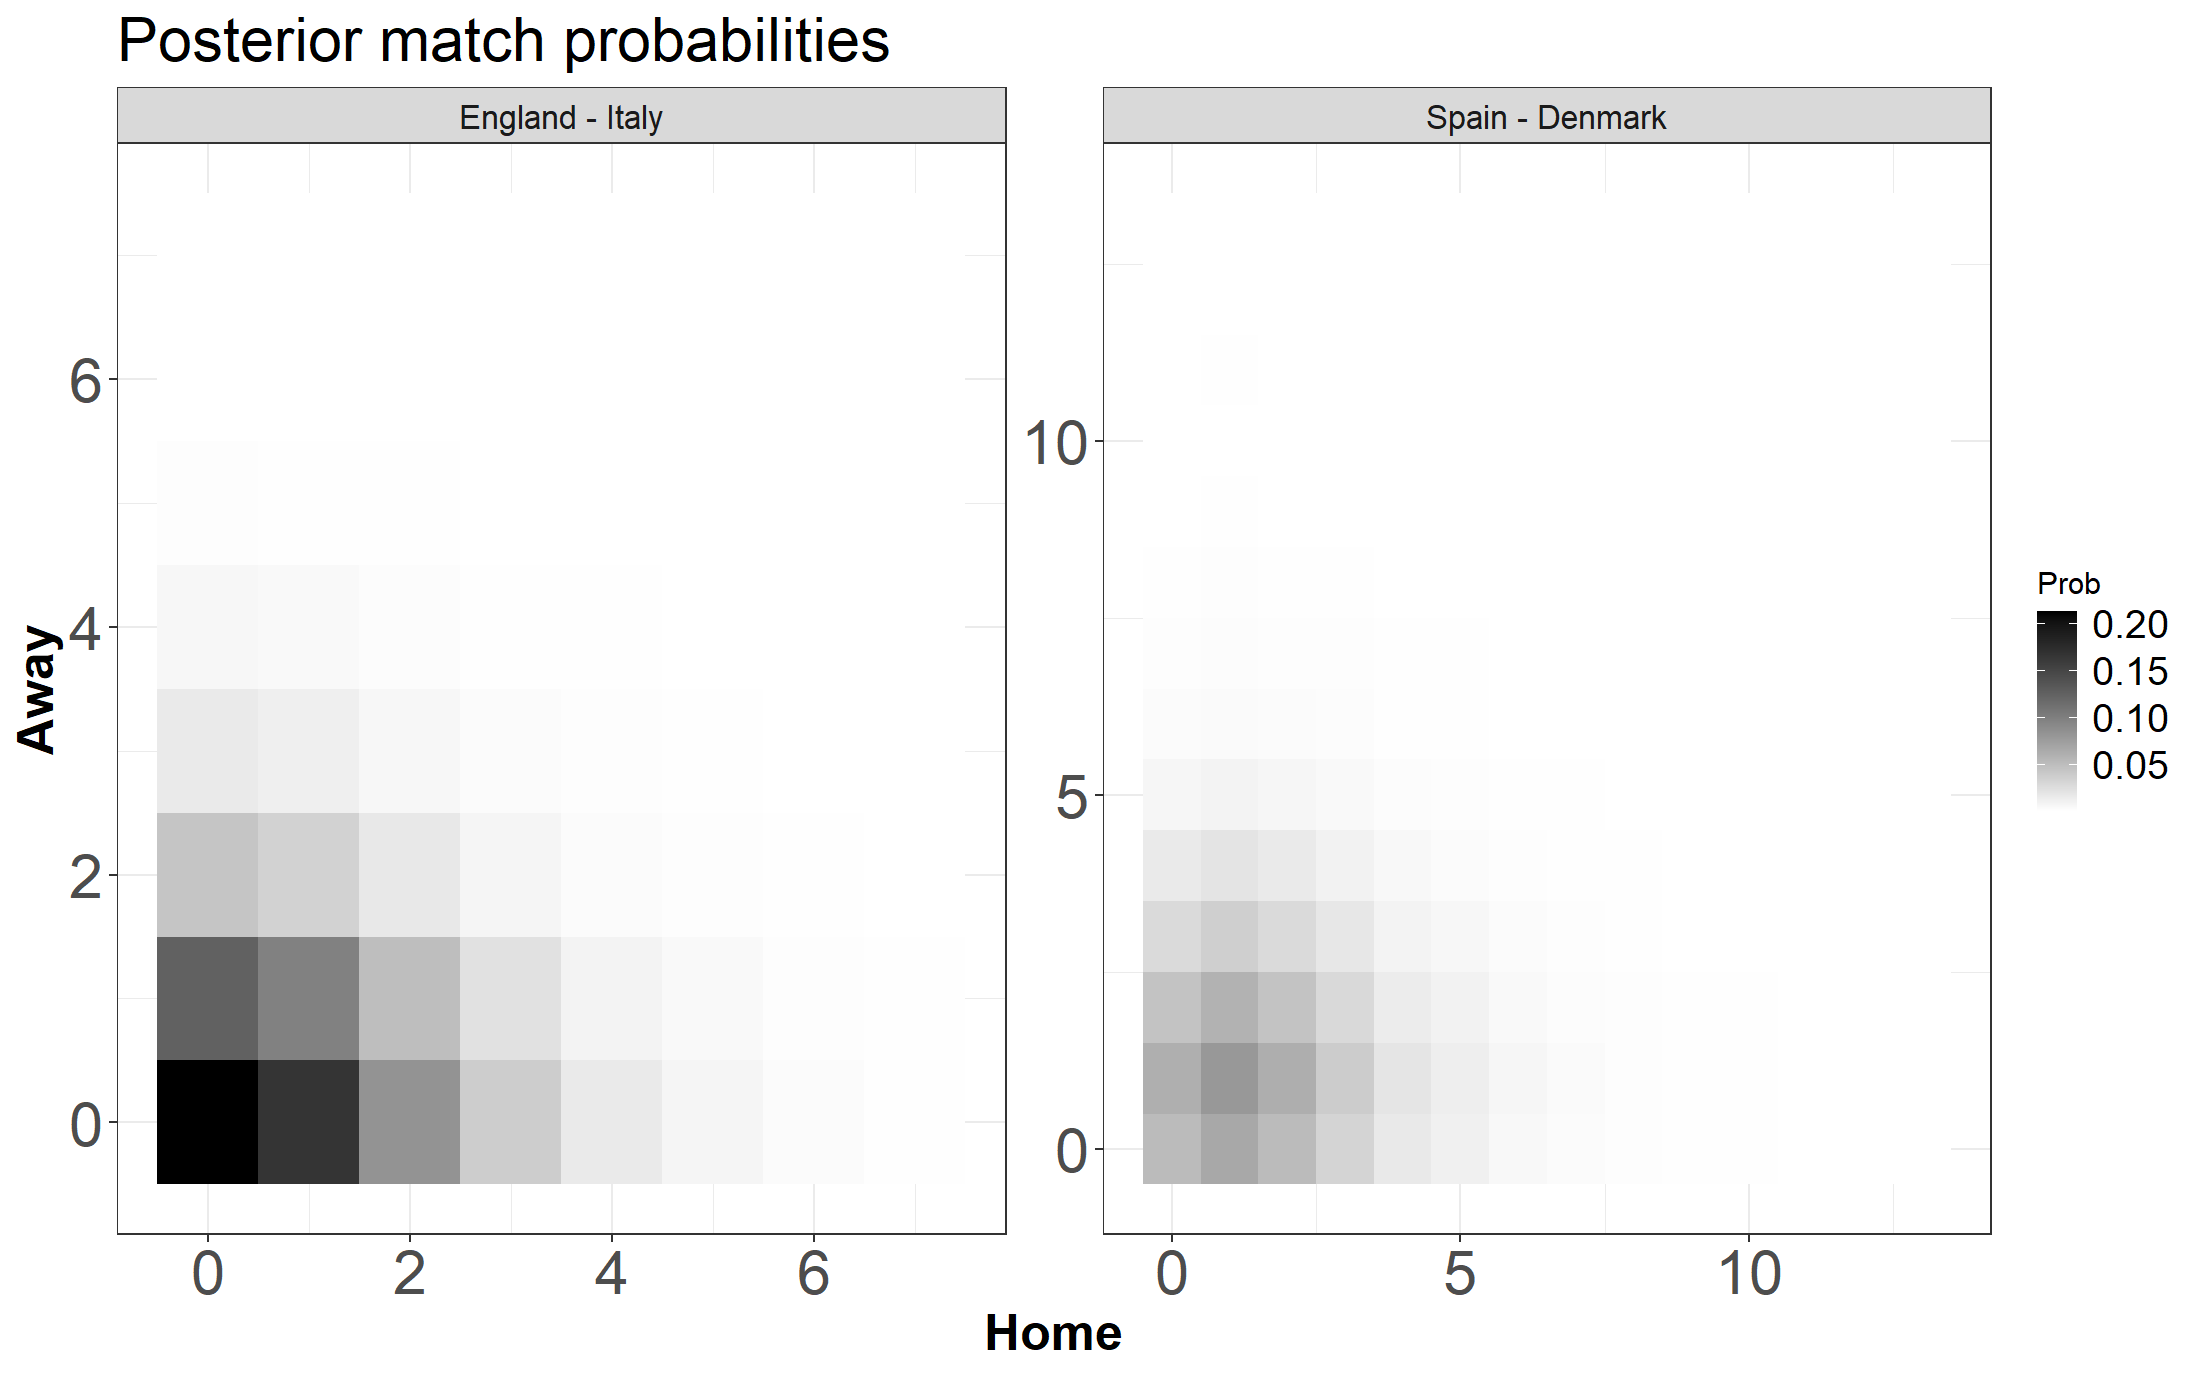
\includegraphics[width=0.8\linewidth]{figs/data2-1} \end{center}

\end{document}
